\section{SQL Injection Mitigation}

Poiché gli attacchi SQL Injection sono così diffusi, dannosi e variegati sia per
via dell'attacco che per tipo, una singola contromisura non è sufficiente.
Piuttosto un insieme integrato di tecniche è necessario. Le contromisure possono
essere classificate in tre tipi: \textit{Defensive Coding}, \textit{Detection},
e \textit{Run-time Prevention}.

\begin{figure}[H]
    \centering
    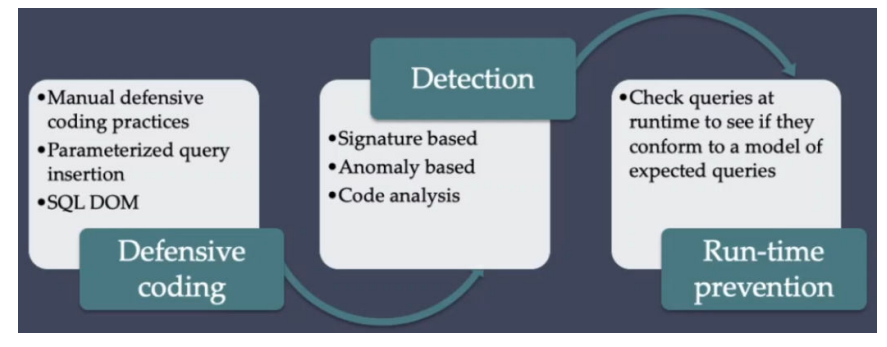
\includegraphics[width=12cm, keepaspectratio]{capitoli/sql_security/imgs/sql2.png}
\end{figure}

\paragraph{Defensive Coding:}
\begin{itemize}
    \item \textbf{Pratiche manuali di codifica difensiva}: Una vulnerabilità
          comune sfruttata da SQL Injection è l'insufficiente convalida
          dell'input. La soluzione semplice per eliminare queste vulnerabilità
          è applicare adeguate pratiche di codifica difensiva. Un esempio è il
          controllo del tipo di input, per verificare che gli input che si
          suppone siano essere numerici non contengano caratteri diversi dalle
          cifre. Questo tipo di tecnica può evitare attacchi basati sulla
          forzatura di errori nel sistema di gestione del database.Un altro
          tipo di pratica di codifica è quella che esegue il pattern matching
          per cercare di distinguere l'input normale da quello anormale.
    \item \textbf{Inserimento di query parametrizzate}: Questo approccio cerca
          di prevenire l'SQL Injection permettendo allo sviluppatore
          dell'applicazione di specificare più accuratamente la struttura di
          una query SQL, e passare i parametri di valore ad essa separatamente
          in modo che qualsiasi input dell'utente non possa
          modificare la struttura della query.
    \item \textbf{SQL DOM}: è un insieme di classi che permette la
          validazione automatica del tipo di dati, la validazione e l'escape.
          Questo approccio usa l'incapsulamento delle query di database per
          fornire un modo sicuro e affidabile per accedere ai database. Questo
          cambia il processo di costruzione delle query da un processo non
          regolamentato che usa la concatenazione di stringhe ad uno
          sistematico che utilizza un'API controllata.
\end{itemize}

\paragraph{Detection:}
\begin{itemize}
    \item \textbf{Signature based}: Questa tecnica tenta di rilevare specifici
          pattern di attacco in quanto ogni tipologia di attacco presenta
          un'esecuzione simile. Similmente agli antivirus questa contromisura
          deve essere costantemente aggiornata in quanto cambiare anche di pochissimo
          il pattern di attacco potrebbe renderlo non rilevabile.
    \item \textbf{Anomaly Based}: Questo approccio tenta di definire il
          comportamento normale e poi rilevare i modelli di comportamento al
          di fuori della gamma normale. C'è una fase di
          addestramento, in cui il sistema impara la gamma di comportamenti
          normali, seguita dalla fase di rilevamento vera e propria.
    \item \textbf{Code Analysis}: Le tecniche di analisi del
          codice coinvolgono l'uso di una suite di test per rilevare le
          vulnerabilità. La suite di test è progettata per generare una
          vasta gamma di attacchi e valutare la risposta del sistema.
\end{itemize}

\paragraph{Run-time Prevention:}
Queste tecniche controllano le query in fase di esecuzione per vedere se risultano
conformi ad un modello di query attese. Sono disponibili vari strumenti
automatizzati per questo scopo.